\begin{figure}

    \centering
    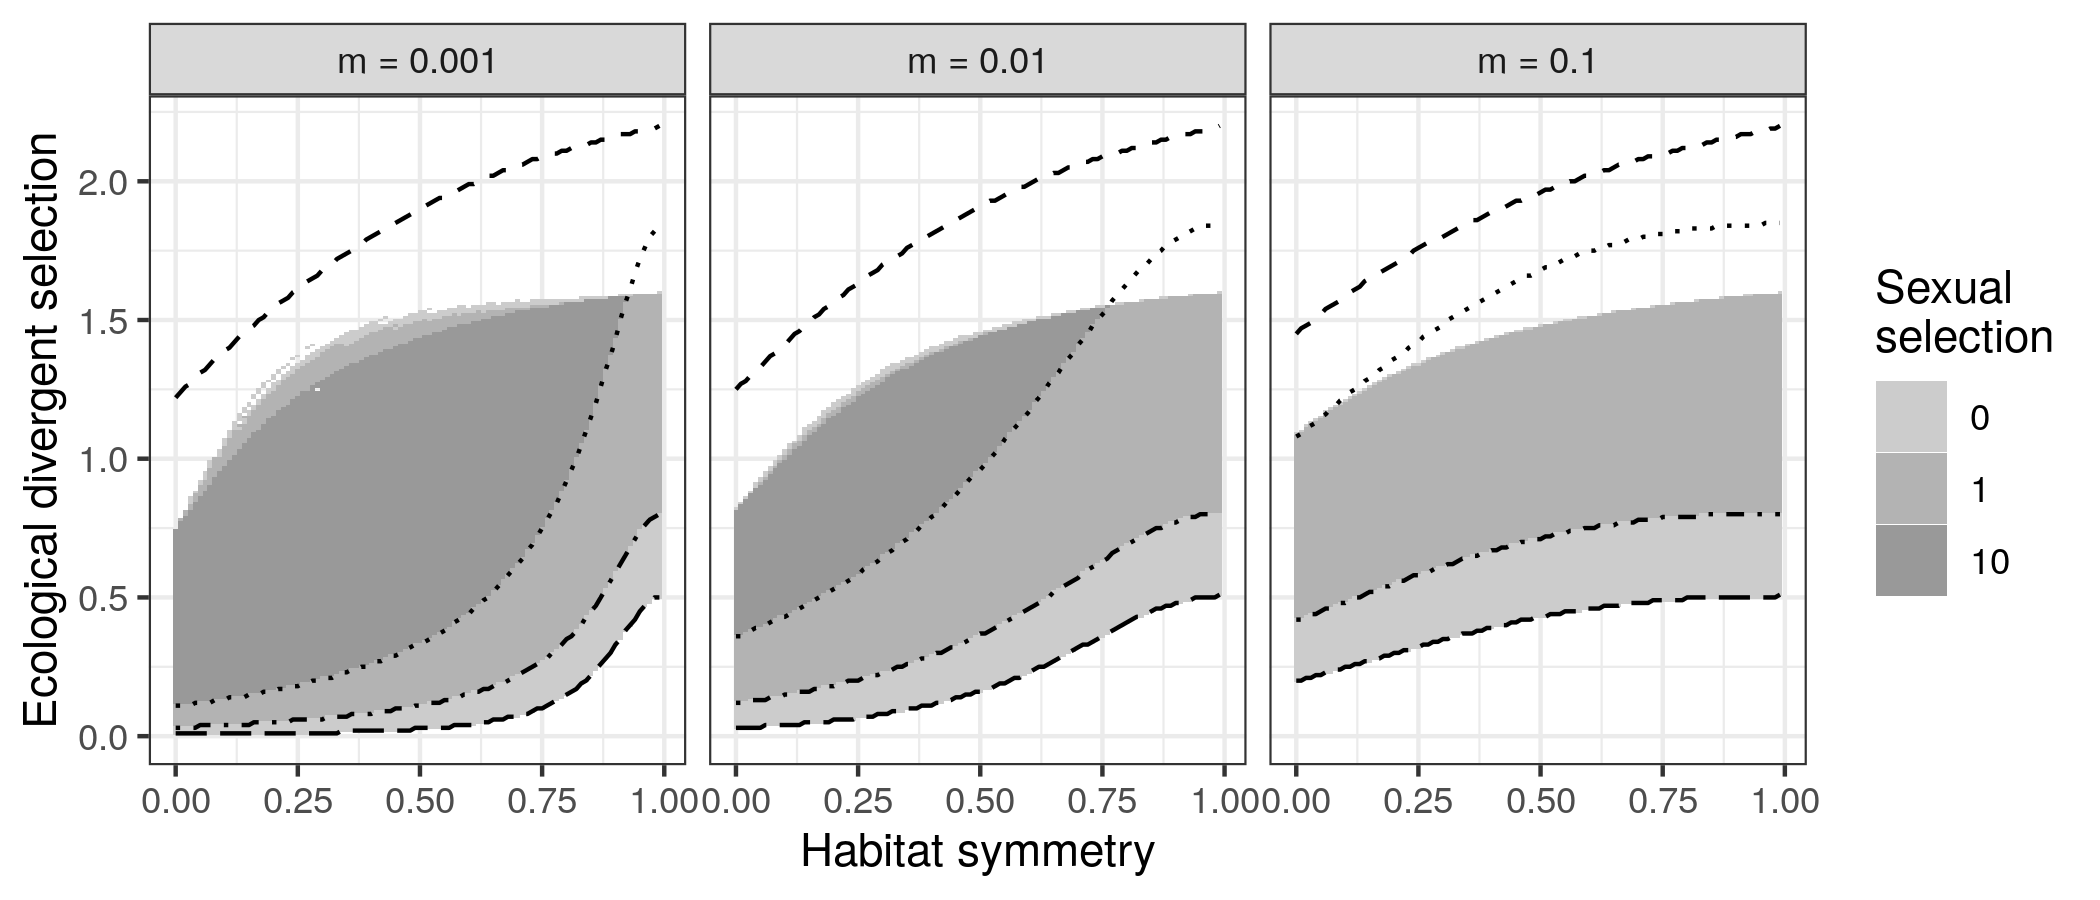
\includegraphics[width=\textwidth]{figures/map_branching_points}
    \caption{Branching throughout parameter space for three values of the dispersal rate $m$. Sexual selection increases the stability of evolutionary equilibria and therefore turns branching points into stable strategies. Shades of grey indicate the highest tested level $\alpha$ of sexual selection at which branching still occurs when a population is initially a specialist of the first resource ($x = -1$). Dashed lines expand the borders of the grey areas to show the full extent of where branching can theoretically occur, irrespective of the starting trait value.}
    \label{fig:map_branching_points}
    
\end{figure}

\begin{figure}

    \centering
    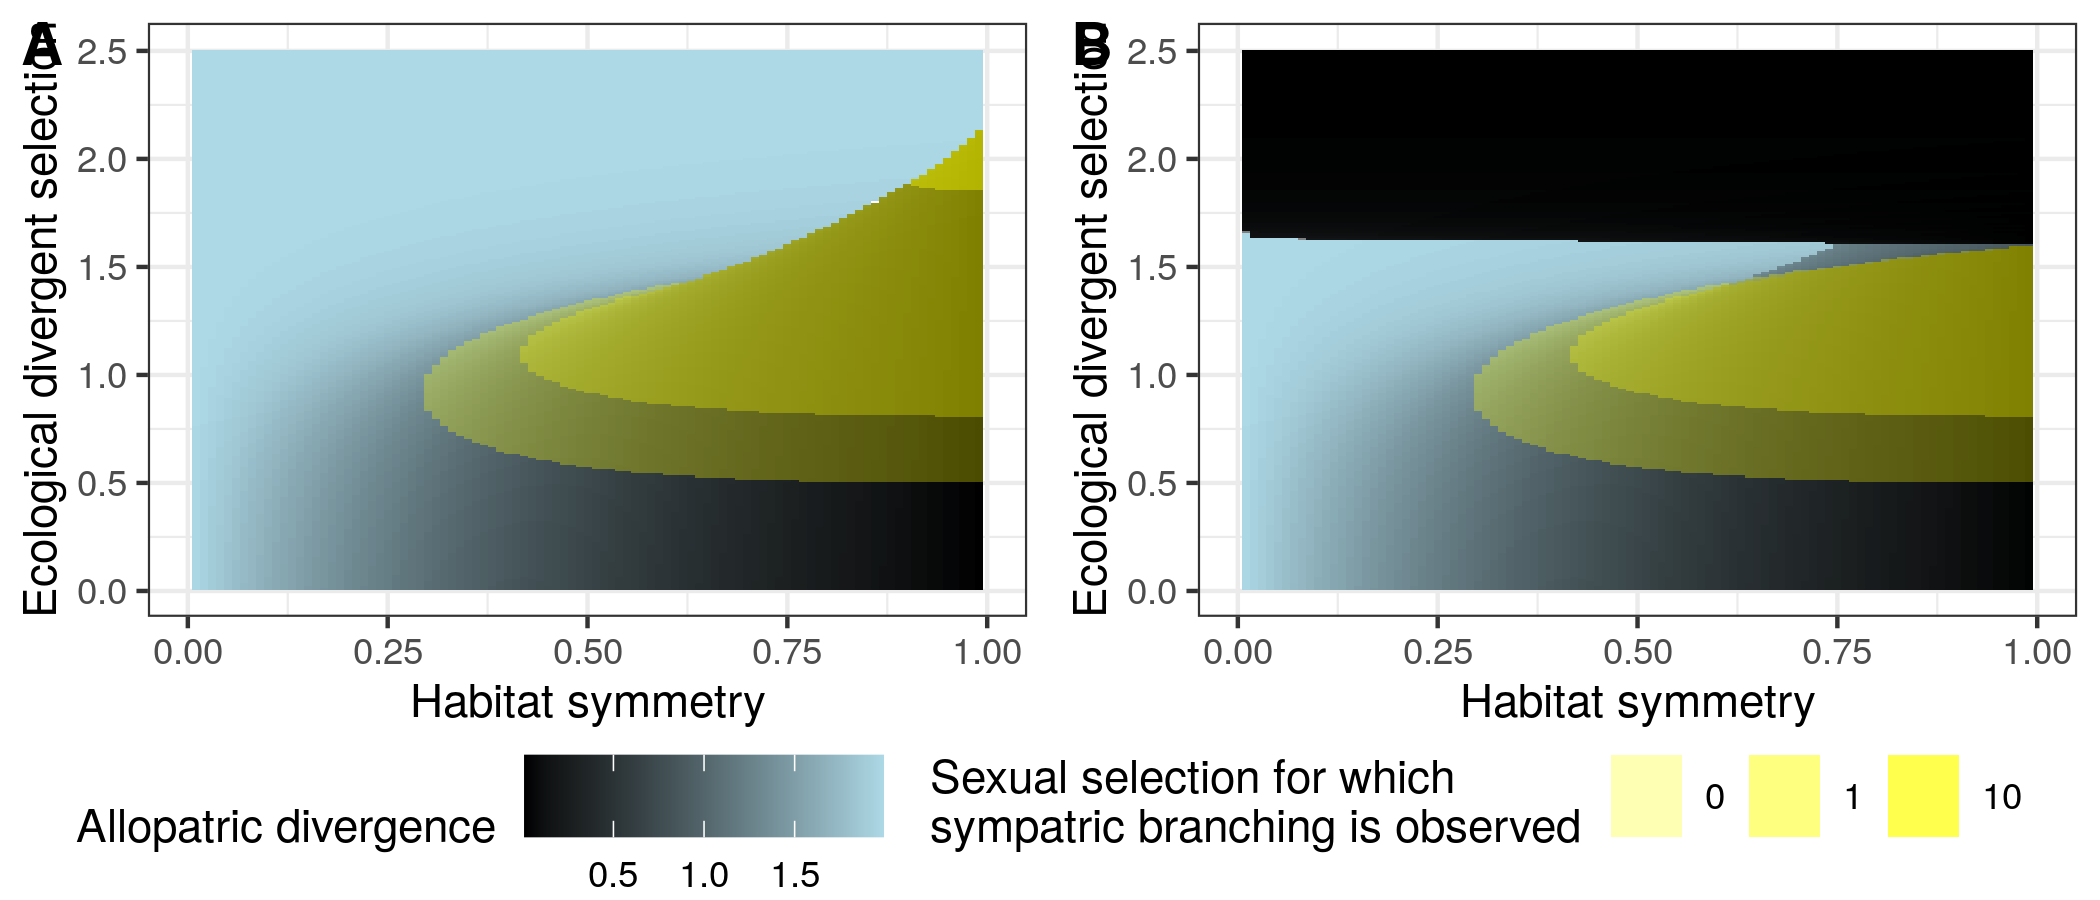
\includegraphics[width=\textwidth]{figures/divergence_across_patches}
    \caption{Adaptive dynamics of a mode without dispersal, for two different starting points. In the absence of dispersal, one can disentangle the effect of local adaptation, i.e. the divergence in equilibrium trait value that occurs in allopatry (shades of blue), and competition, i.e. whether branching occurs in sympatry, within each patch (yellow transparent layer). Starting trait values: (A) $x = 0$, (B), $x = -1$.}
    \label{fig:map_divergence}
    
\end{figure}